\documentclass[a4paper, 11pt, notitlepage]{article}

% \usepackage[norsk]{babel}
\usepackage{textcomp}
\usepackage[utf8]{inputenc}
\usepackage[T1]{fontenc, url}
\usepackage{amsmath, amssymb}
\usepackage{amsbsy, amsfonts}
\usepackage{graphicx, color, xcolor}
\usepackage{framed, parskip, titling}
\usepackage{flafter, caption, multicol}
\usepackage{verbatim, listings}
\usepackage{shadow}
\usepackage{url}
\usepackage{framed}
\usepackage{fancyvrb}
\usepackage{titling}


%\DeclareCaptionLabelSeparator{colon}{. }
\renewcommand{\captionfont}{\sffamily}
\renewcommand{\captionlabelfont}{\bf\sffamily}
\setlength{\captionmargin}{40pt}

\setcounter{tocdepth}{2}

% \lstset{language=c++}
% \lstset{basicstyle=\footnotesize\sffamily,
%   numbers=left,                   % where to put the line-numbers
%   numberstyle=\tiny\color{gray},  % the style that is used for the line-numbers
%   stepnumber=2, }
% \lstset{backgroundcolor=\color{white}}
% \lstset{frame=single}
% \lstset{stringstyle=\sffamily}
% \lstset{keywordstyle=\color{red}\bfseries}
% \lstset{commentstyle=\color{blue}}
% \lstset{showspaces=false}
% \lstset{showstringspaces=false}
% \lstset{showtabs=false}
% \lstset{tabsize=2}
% \lstset{breaklines}

\definecolor{javared}{rgb}{0.6,0,0} % for strings
\definecolor{javagreen}{rgb}{0.25,0.5,0.35} % comments
\definecolor{javapurple}{rgb}{0.5,0,0.35} % keywords
\definecolor{javadocblue}{rgb}{0.25,0.35,0.75} % javadoc

\lstset{language=c++,
basicstyle=\ttfamily\footnotesize,
keywordstyle=\color{javapurple}\bfseries,
stringstyle=\color{javared},
commentstyle=\color{javagreen},
morecomment=[s][\color{javadocblue}]{/**}{*/},
numbers=left,
numberstyle=\tiny\color{black},
stepnumber=2,
numbersep=10pt,
tabsize=2,
showspaces=false,
showstringspaces=false,
frame= single,
breaklines=true}

\usepackage{geometry}
\geometry{headheight=0.01mm}
\geometry{top=24mm, bottom=29mm, left=39mm, right=39mm}

\renewcommand{\arraystretch}{2}
\setlength{\tabcolsep}{10pt}
% \makeatletter
% \renewcommand*\env@matrix[1][*\c@MaxMatrixCols c]{%
%   \hskip -\arraycolsep
%   \let\@ifnextchar\new@ifnextchar
%   \array{#1}}
% \makeatother

\newcommand{\dd}[1]{\ \text{d}#1}
\newcommand{\f}[2]{\frac{#1}{#2}} 
\newcommand{\beq}{\begin{equation}}
\newcommand{\eeq}{\end{equation}}
\newcommand{\bra}[1]{\langle #1|}
\newcommand{\ket}[1]{|#1 \rangle}
\newcommand{\braket}[2]{\langle #1 | #2 \rangle}
\newcommand{\av}[1]{\left| #1 \right|}
\newcommand{\op}[1]{\widehat{#1}}
\newcommand{\braopket}[3]{\langle #1 | \op{#2} | #3 \rangle}
\newcommand{\ketbra}[2]{\ket{#1}\bra{#2}}
\newcommand{\pp}[1]{\frac{\partial}{\partial #1}}
\newcommand{\ppn}[1]{\frac{\partial^2}{\partial #1^2}}
\newcommand{\up}{$\uparrow$}
\newcommand{\down}{$\downarrow$}
\newcommand{\bt}[1]{\boldsymbol{#1}}
\newcommand{\mat}[1]{\textsf{\textbf{#1}}}
\newcommand{\I}{\boldsymbol{\mathcal{I}}}
\renewcommand{\d}{{\rm d}}

\makeatletter
\renewcommand*\env@matrix[1][*\c@MaxMatrixCols c]{%
  \hskip -\arraycolsep
  \let\@ifnextchar\new@ifnextchar
  \array{#1}}
\makeatother

\title{{\centerline{\Huge Laboratorieoppgave:}} \vspace{0.4cm} {\centerline{\Huge Elektron Spinn Resonans}} \vspace{0.4cm} {\centerline{\LARGE FYS3710}}}
\author{Kandidatnummer 303}
\setlength{\droptitle}{2.5cm}

\begin{document}
\maketitle


\vspace*{3.5cm}

\begin{abstract}
Denne laboratorieoppgaven dreier seg om bruk av ESR/EPR spektroskop. Oppgaven er todelt. Del a) handler om bruk av EPR/ESR til deteksjon av frie radikaler i bestrålt vann og tungtvann. Hyperfinkonstanten for hydrogen- og deuteriumatomer, samt noen andre fysiske størrelser, bestemmes empirisk gjennom forsøket og sammenlignes med kjente teoretiske verdier. Del b) er et forsøk på dosebestemmelse av bestrålte nitroglyserintabletter fra Kjellerulykken 1982. Her sammenlignes fire prøver bestående av samme type pulver, tre av prøvene er blitt bestrålt med en kjent dose, den siste har blitt bestrålt med en ukjent dose. Bruk av intensitetssammenligninger av ESR/EPR-spektrene fra de fire prøvene lar oss estimere dosen den ukjente prøven er blitt utsatt for.
\end{abstract}

\clearpage

\section{Bakgrunn}
Elektron paramagnetisk resonans (EPR), også kalt elektron spinn resonans (ESR), spektroskopi er en måleteknikk for paramagnetiske prøver. Prøver som inneholder molekyler med uparede elektroner vil nødvendigvis være paramagnetiske, og egner seg derfor meget godt til studie gjennom EPR/ESR spektroskopi.

Prinsippet bak EPR/ESR spektroskopi har mye til felles med NMR. Hovedforskjellen på de to teknikkene er at det er kjernespinn som eksiteres i NMR, mens det for EPR/ESR er elektronspinnet.

Elektroner er spinn-$1/2$ partikler, som betyr at de kan innta to lineært uavhengige spinntilstander, $m_s = \pm 1/2$. Ettersom at elektronet har både spinn og ladning, har det et magnetisk moment $\mu = -g\beta\vec{S}$. Når vi fører elektronet inn i et ytre magnetfelt, vil elektronets magnetiske moment orientere seg enten parallelt eller antiparallelt med feltets retning, disse to tilstandene kalles gjerne for ``spinn opp'' og ``spinn ned''. På grunn av Zeeman-effekten vil de to tilstanden ha en energidifferanse på
$$\Delta E = g\beta B,$$
for å eksitere en overgang fra lav til høy tilstand bestråler vi prøven med elektromagnetisk stråling med fotonenergi lik energidifferansen
$$h\nu = \Delta E = g\beta B,$$
dette er resonansbetingelsen for EPR/ESR spektroskopi og er grunnlaget for hele metoden.

Vi setter prøven inn i et magnetisk felt med konstant retning, men varierende feltstyrke. Vi bestråler prøven kontinuerlig med EM-stråling med en gitt frekvens $\nu$. Vi varierer så feltstyrken $B$, og måler hvor mye stråling prøven absorberer ved forskjellige feltstyrker. Når resonansbetingelsen er oppfylt vil vi ha nett absorbsjon av EM-stråling i prøven, men ellers ikke. Fra intensiteten til energiabsorpsjonen kan vi også få informasjon om antallet uparede elektroner i prøver.

\section{Metode}
\subsection{a) Deteksjon av frie radikaler i bestrålt vann og tungtvann}
En løsning av svovelsyre, vann (H$_2$O) og tungtvann (D$_2$O) fryses til kuler på omtrent 1 mm og oppbevares i flytende nitrogen (N$_2$) for å holde temperaturen lav. Prøven bestråles så med ioniserende Röntgenstråling for å danne frie radikaler i form av hydrogenatomer og deuteriumatomer (H$\bullet$, D$\bullet$). Ved romtemperatur ville disse frie radikalene være kortlevde og vanskelig å observere, men ettersom at prøven holdes kaldt kan den flyttes til prøvekammeret i ESR/EPR maskinen. ESR/EPR spektroskopi utføres så på prøven og spekteret taes opp.

\subsection{b) Dosebestemmelse av bestrålte nitroglyserintabletter}
Det benyttes 4 prøver med pulver fra knuste nitroglyserintabletter, der tre har blitt utsatt for en kjent dose. Den siste prøven er utsatt for en ukjent dose. Det utføres ESR/EPR spektroskopi på alle fire prøvene etter tur, og spekteret taes opp. Fra de relative amplitudene til de tre kjente prøvene lager vi en kalibreringskurve som brukes til å estimere dosen den ukjente prøven er utsatt for.

\section{Resultater}

\subsection{a) Deteksjon av frie radikaler i bestrålt vann og tungtvann}

Vi får et 1.\ derivert absorpsjonsspekter for prøven vår. Dette spekteret er lagt ved som vedlegg a). Her måler vi av nullpunktene som svarer til absorpsjonstoppene. Vi måler bare av feltstyrken der resonans finner sted, den relative absorpsjonsintensiteten er uviktig i dette tilfellet. Ved $B_0$, dvs, i ``midten'' av spekteret, er det ganske kaotiske målinger, dette er blant annet pågrunn av støy fra sulfationene som er i prøven. Vi prøver derfor ikke å måle $B_0$ verdiene direkte fra midten av spekteret, men leser bare av $B$-verdiene for de fire andre toppene.

De målte verdiene er
\begin{center}
\begin{tabular}{c}
3134,70 Gauss \\
\hline
3328,32 Gauss \\
\hline
3483,32 Gauss \\
\hline
3641,78 Gauss
\end{tabular}
\end{center}

\subsection{b) Dosebestemmelse av bestrålte nitroglyserintabletter}
Vi lager fire 1.\ deriverte absorpsjonsspektre. For hver av spektrene leser vi av den relative forskjellen i amplituden til den største toppen og bunn, og den minste toppen og bunn. I dette tilfellet er den magnetiske feltstyrken uviktig. For et eksempel på et av absorpsjonsspektrene, se vedlegg b), som er resultatet fra en av prøvene. De målte verdiene er
\begin{center}
\begin{tabular}{l|c|c}
Prøve & $\Delta_{\rm min}$ & $\Delta_{\rm max}$ \\
68 Gy & 1.7484$\cdot10^5$ & 3.1225$\cdot10^5$ \\
20 Gy &	7.0455$\cdot10^4$ & 1.15653$\cdot10^5$ \\
10 Gy &	4.8664$\cdot10^4$ & 7.2422$\cdot10^4$ \\
Ukjent & 1.27897$\cdot10^5$ & 2.2415$\cdot10^5$
\end{tabular}
\end{center}

\clearpage 

\section{Diskusjon}

\subsection{a) Deteksjon av frie radikaler i bestrålt vann og tungtvann}

\subsubsection{Energier}
Energinivåene for elektronenenes spinntilstander splittes som følge av to forskjellige effekter, det er elektron-Zeemanvekselvirkningen, som vil si energiforskjellen som oppstår som følge av elektronets magnetiske moment iforhold til det ytre magnetfeltet. Og det er vekselvirkningen mellom elektronets og kjernens magnetiske momenter. Etter disse splittingene vil hyperfinstrukturen endre energinivåene litt yttligere, men vil ikke føre til mer splitting av nivåer.

For hydrogen har vi et kjernespinn på $I=1/2$, som betyr at elektron-kjerne vekselvirkningen splitter hvert energinivå i to. For deuterium har vi et kjernespinn på $I=1$, som betyr at elektron-kjerne vekselvirkningen splitter hvert energinivå i tre. Se figur 1 og 2 på neste side for å se hvordan energidiagrammene for de to atomene ser ut.

EPR/ESR overganger er et flip i elektronets spinntilstand, vi har altså utvalgsregler
$$\Delta m_s = \pm 1, \qquad \Delta m_I = 0.$$
Vi ser da fra figur 1 og 2 at det for hydrogenatomet er to tilatte overganger. Energiforskjellen på disse to overgangene blir
$$\Delta E = a'.$$
For deuteriumatomet ser vi at det er tre tilatte overganger, med en lik energiforskjell på $a'$ mellom hvert steg, slik at det blir $2a'$ energiforskjell mellom den minste og den største overgangen. Dette vil si at vi forventer å se to linjer fra hydrogenatomet, og tre linjer fra deuteriumatomet i ESR/EPR spekteret.


\begin{figure}[p]
\centering
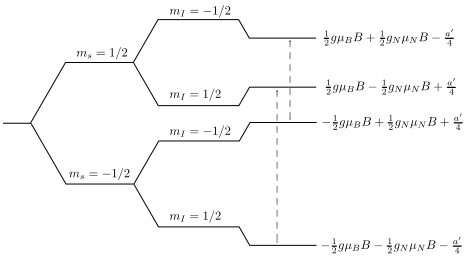
\includegraphics[width=\textwidth]{fig_1.pdf}
\caption{Energidiagram for spinntilstandene i hydrogen, H$\bullet$.}
\end{figure}
\begin{figure}[p]
\centering
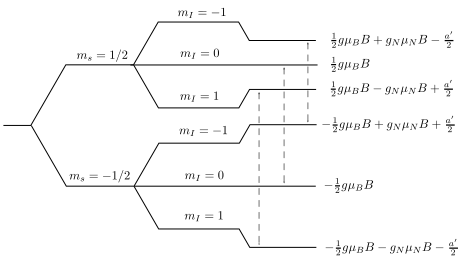
\includegraphics[width=\textwidth]{fig_2.pdf}
\caption{Energidiagram for spinntilstandene i et deuterium, D$\bullet$.}
\end{figure}


\subsubsection{Hyperfinsplitting}
Fra resultatene kan vi prøve å estimere hyperfinsplittingskonstantene til hydrogen og deuterium $a_{\rm H}$ og $a_{\rm D}$. Vi vil spesielt se på forholdet av disse, da dette forholdet lett kan regnes ut teoretisk
$$\frac{a_{\rm H}}{a_{\rm D}} = \frac{\frac{2\mu_0}{3} g_{\rm H} \beta |\Psi(r_N)|^2}{\frac{2\mu_0}{3}g_{\rm D} \beta |\Psi(r_N)|^2}.$$
Så vi ser at forholdet mellom hyperfinsplittingene er lik forholdet mellom spektroskopiske splittingsfaktorene, slik at
$$\frac{g_{\rm H}}{g_{\rm D}} = \frac{5.585}{0.857} = 6.517.$$

Fra de målte verdiene fra vedlegg 1 fant vi at
$$2a_{\rm D} = 155 \mbox{ Gauss}, \qquad a_{\rm H} = 507.08 \mbox{ Gauss}.$$
det betyr at vi har målt forholdet mellom hyperfinsplittingene til å være
$$a_{\rm H} / a_{\rm D} = 507.08/(155/2) = 6.54.$$

Fra resonansbetingelsen vet vi at
$$h\nu = g_e\beta_e B_0,$$
her er $h$ Planck's constant, $\nu$ er frekvensen til ESR/EPR maskinen, som nå er $\nu = 9.5425$ GHz, $\beta_e$ er Bohr magnetonet som er definert som $e\hbar/2m_e$. Vi kan da estimere $g_e$ fra $B_0$. Her er $B_0$ feltverdien midt i mellom de to toppene for hydrogenatomet, og midt mellom de to ytterste toppene for deuteriumatomet. Vi har at
\begin{center}
\begin{tabular}{l|c|c}
 & $B_0$ & $g_e$ \\
\hline
Hydrogen & 3405.82 Gauss & 2.0018 \\
\hline
Deuterium & 3388.24 Gauss & 2.0122 \\
\end{tabular}
\end{center}
Vi ser at $g_e$ blir litt forskjellig for de to forskjellige atomene, dette skyldes 2.\ ordens effekter, noe vi ikke kommer til å diskutere nærmere her.

\subsubsection{Bestemme $|\Psi(r_N)|^2$}

Hyperfinsplittingskonstanten kan uttrykkes som
$$a = \frac{2\mu_0}{3}g_N\beta_B |\Psi(r_N)|^2,$$
der $|\Psi(r_N)|^2$ er sannsynlighetstettheten for elektronet å befinne seg på kjernens plass. Vi skal nå finne denne størrelsen både fra resultatene våres, og teoretisk.

Teoretisk finner vi sannsynligheten fra bølgefunksjonen
$$\Psi(r) = \frac{1}{\sqrt{\pi a_0^3}}e^{-r/a_0},$$
der $a_0$ er Bohr radiusen. Innsetting av $r=r_N = 0$ gir da sannsynlighetstettheten. Vi finner de empirisk målte verdiene ved å manipulere uttrykket for $a$. Finner da at
$$|\Psi(r_N)|^2 = \frac{3a}{2\mu_0 g_N \beta_N},$$
der $\mu_0 = 4\pi\cdot10^{-7}$, $g_N = g_H = 5.585$ for hydrogen og $g_N = g_D = 0.857$ for deuterium, og $\beta_N = e\hbar/2m_p$, der $m_p$ er proton massen. Vi finner da litt forskjellig verdi for hydrogen og deuterium
\begin{center}
 \begin{tabular}{l|c}
             & $|\Psi(r_N)|^2$ \\ \hline
 Teoretisk & $2.148 \cdot 10^{30}$ \\ \hline 
 Målt Hydrogen & $2.1457 \cdot 10^{30}$   \\ \hline
 Målt Deuterium & $2.1372 \cdot 10^{30}$
 \end{tabular}
\end{center}

\clearpage


I hvert spekter vil amplituden av 1.\ derivert-spekteret være proporsjonalt med arealet under kurven, som igjen er proporsjonalt med mengden frie radikaler i prøven. Vi opererer med antagelsen at mengden frie radikaler i prøven igjen er proporsjonalt med stråledosen prøven har fått.

Vi kjører en lineær regresjon på måledataene vha Casio kalkulator, og finner to linjer, den ene for de minste toppene i spekteret, og en for de største toppene i spekteret. I begge tilfeller er $r^2 > 0.9999$, så de tre prøvene ligger på en rett linje, som forventet. Fra disse finner vi den estimerte stråledosen til de målte amplitudene på den ukjente prøven. Vi finner da følgende tall
\begin{center}
 \begin{tabular}{l|c}
             & Dose fra ukjent prøve \\ \hline
 Fra $\Delta_{\rm min}$ & 46.4 Gy \\ \hline 
 Fra $\Delta_{\rm max}$ & 46.6 Gy\\ \hline
 Snitt & 46.5 Gy
 \end{tabular}
\end{center}

\subsubsection{Feilkilder}
Ettersom at vi sammenligner relative amplituder, er det ekstremt viktig at EPR/ESR maskinen er stillt inn med like parametere for hver av de fire prøvene. Om noen av disse parameterene endres, så vil amplituden på det påfølgende spekteret heller ikke kunne sammenlignes med de andre spektrene. Det er også viktig at de fire måleprøvene har samme mengde pulver. Dette er fordi vi sammenligner mengden frie radikaler i det systemet, slik at en større prøve nøvendigvis vil inneholde flere radikaler. Vi hadde ingen mulighet til å være sikre på at prøvene var av like mengder, så dette blir en betydelig feilkilde på sluttresultatet.


\section{Konklusjon}
\subsection{a) Deteksjon av frie radikaler i bestrålt vann og tungtvann}
Vi har sett at ved å måle ved hvilke feltstyrker prøven absorberer stråling ved en kjent frekvens har gitt oss mulighet til å regne ut diverse empiriske størrelser, både for hydrogenatomet og deuteriumatomet. Vi har sett at disse verdiene har vært i forholdsvis god overensstemmelse med kjente teoretiske verdier.

\subsection{b) Dosebestemmelse av bestrålte nitroglyserintabletter}
Den estimerte dosen den ukjente prøven hadde blitt utsatt for var 46.5 Gy. LD-50, det vil si den dosen der 50 \% av en befolkningen ikke overlever 30 dager anslåes til å være ca. 5 Gy, og dose ved beinmargstransplantasjon, som er en meget drastisk behandling, er 10 Gy i helkroppsdose. Etter å ha fått en dose på over 40 Gy, kan det derfor med rimelig sikkerthet anslåes at det var null overlevelsessannsynlighet, selv med akkutt behandling.




\end{document}
